\chapter{Results}
\label{chap:Results}
\paragraph*{}
From the design given in the previous chapter \ref{chap:theory}, two implementations are created. One without scanline buffers, and the other with scanline buffering. In the following sections, the results from the simulation, synthesis and hardware testing of theses implementations will be presented and discussed. \\
To ensure that the generated results are correct, a Matlab verification script is created (appendix \ref{app:Matlab}). The script contains a reference calculation of the Sobel filter, that mimics the expected and desired operation of the VHDL implementation.
The calculated reference, is subsequently compared with output image generated by either the simulation or the hardware test.

\section{Implementation of Sobel operator without scanline buffering.}
\paragraph*{}
With the design given in the ASM diagram (figure \ref{fig:ASM_HW} in section \ref{sec:AccDesign}, the VHDL source found in appendix \ref{app:acc2} has been implemented. The implementation have been synthesised, simulated and tested on the \textit{Nexys3 board} and the result is successfully verified by the Matlab verification script.\\
Figure \ref{fig:sum_synthesis_report}, shows an extract from the synthesis report that is generated by the \textit{Xilinx  ISE tool}. The inferred Adders and D-flip flops are almost identical to the anticipated values given in tables  \ref{tab:designRegisters} and table \ref{tab:designAdders}.
 
\begin{figure}[H]
\centering
\begin{BVerbatim}
Summary:
    inferred  31 Adder/Subtractor(s).
    inferred 232 D-type flip-flop(s).
    inferred   3 Comparator(s).
    inferred  59 Multiplexer(s).
    inferred   1 Finite State Machine(s).
\end{BVerbatim}
\caption{Summary of synthesis report ISE project navigator}
\label{fig:sum_synthesis_report}
\end{figure}

\textcolor{red}{ToDo: Maximum Clock rate ??}

\paragraph*{}
Before the design have been implemented on the Nexys board a simulation with ModelSim have been preformed on a image of a roller coaster with $352x288$ pixels see figure \ref{fig:test_picture_raw}. 

\begin{figure}[H]
	\centering
	\begin{subfigure}[b]{0.4\textwidth}
		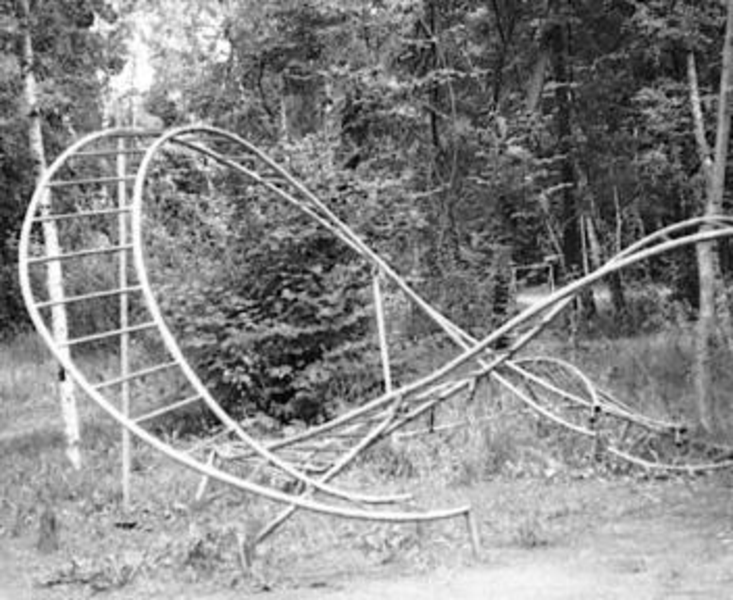
\includegraphics[width=1 \textwidth]{raw.pdf}
		\caption{Raw image before simulation}
		\label{fig:test_picture_raw}
    \end{subfigure}%
        ~ %add desired spacing between images, e. g. ~, \quad, \qquad, \hfill etc. 
    \begin{subfigure}[b]{0.4\textwidth}
    	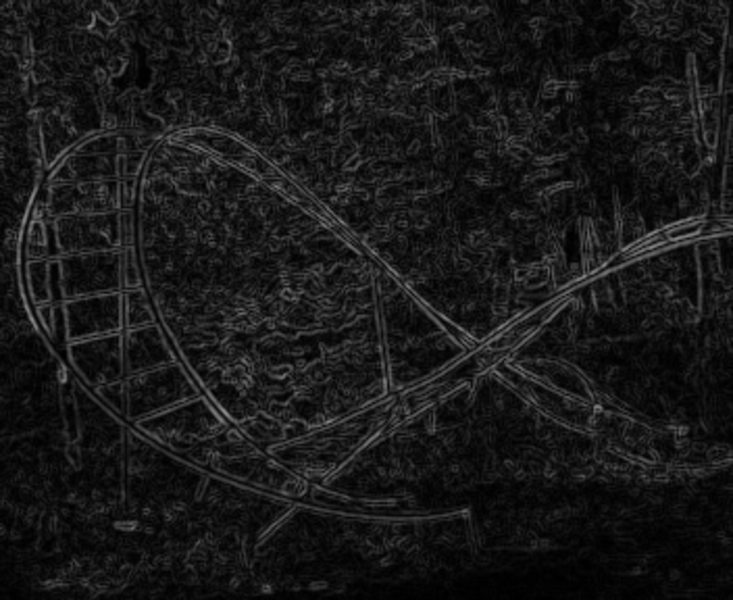
\includegraphics[width=1 \textwidth]{sobel_result.pdf}
    	\caption{After simulation}
    	\label{fig:test_picture_sobel}
	\end{subfigure}
	\caption{Scanline buffering of pixel data.}
\end{figure}

\paragraph*{}
The simulation was completed after $24.4ms$ which result gives a calculation range of $40.9$ $frames~pr.~sec$ or $4.15Mpix/sec$ which is in accordance with the estimations in section \ref{sec:AccDesign}. A section of the waveform from the simulation can be seen in figure ??. The edge detected picture in figure \ref{fig:test_picture_sobel} have been check and verified with the MATLAB verfication script found in appendix \ref{app:Matlab}.   

\section{Optimization with scanline buffers}
\paragraph*{}
In the section \ref{sec:Optimization} the scanline buffer design was described. As well as with the basic design, the scanline buffer design have been synthesised, tested and implemented. Since this design goes along with the basic design but utilizes a dual block ram the synthesis report gives roughly the same amount of a logic components. See figure \ref{fig:sum_synthesis_report_scan} and \ref{fig:sum_synthesis_report_ram}.   
    
\begin{figure}[H]
\centering
\begin{BVerbatim}
Summary:
    inferred  34 Adder/Subtractor(s).
    inferred 230 D-type flip-flop(s).
    inferred   5 Comparator(s).
    inferred  75 Multiplexer(s).
    inferred   1 Finite State Machine(s).
\end{BVerbatim}
\caption{Summary of synthesis report ISE project navigator}
\label{fig:sum_synthesis_report_scan}
\end{figure}

\begin{figure}[H]
\centering
\begin{BVerbatim}
    DATA_WIDTH = 16
    ADDR_WIDTH = 9
    Found 512x16-bit dual-port RAM <Mram_mem> for signal <mem>.
    Summary:
	inferred   1 RAM(s).
	inferred  32 D-type flip-flop(s).
\end{BVerbatim}
\caption{Summary of synthesis report ISE project navigator}
\label{fig:sum_synthesis_report_ram}
\end{figure}

\paragraph*{}
The simulation of the design have shows the scanline design is improved with only one read transaction per pixel as describe in section \ref{sec:Optimization}. This is proven by the fact the simulation complets after $8.29ms$ which roughly is 3 times faster then the basic design and gives a calculation rate of $120$ \textit{frames pr second} or $12.2Mpix/sec$. As with the basic result the scanline result have been verified with the MATLAB script. In figure ?? a section of the waveform  for the scanline design can be seen.

\section{Optimizations using scanline buffers and burst operation of external RAM}
\paragraph*{}
A further optimization where the extern ram is accessed in burst mode was planed. Some simulation result was obtained but getting a working and verified burst mode optimization within the project time frame have not been possible. In figure \ref{fig:burst_picture} the obtained result is seen the red blobs indicate errors. The problem is that the wait period at every $128word$ reads gives a \textcolor{red}{problem with the pixelbuffers saveing a non exiting pixel this is seen from the image of the errors seen in figure \ref{fig:pic_burst_err}.} is this correct??. The burst optimization was expected to have a calculation rate of $26.7Mpix/sec$ but this is not confirmed by simulation or implementation.
     
\begin{figure}[H]
	\centering
	\begin{subfigure}[b]{0.5\textwidth}
		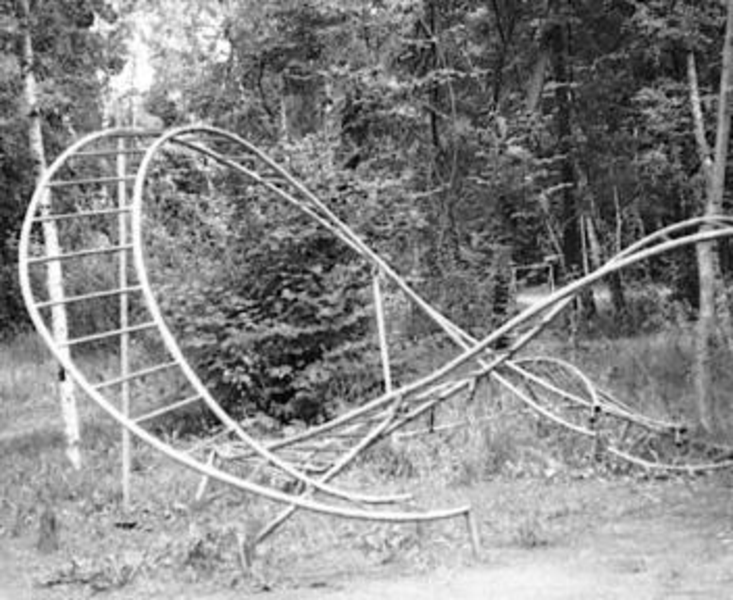
\includegraphics[width=1 \textwidth]{raw.pdf}
		\caption{Raw image before simulation}
		\label{fig:raw_burst}
    \end{subfigure}%
        ~ %add desired spacing between images, e. g. ~, \quad, \qquad, \hfill etc. 
    \begin{subfigure}[b]{0.5\textwidth}
    	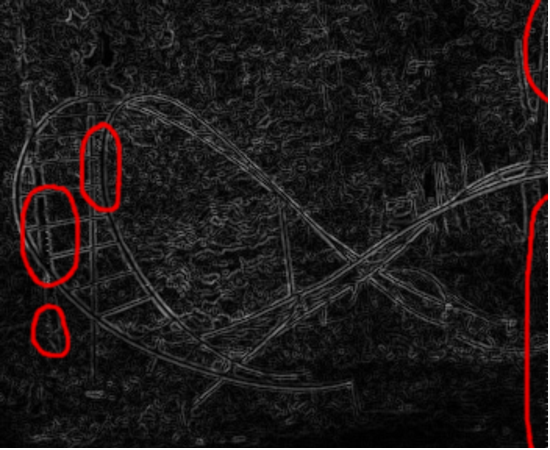
\includegraphics[width=1 \textwidth]{burst_result.pdf}
    	\caption{After simulation red blobs indicated errors}
    	\label{fig:burst_picture_sobel}
	\end{subfigure}
	\caption{Scanline buffering of pixel data.}
    	\label{fig:burst_picture}
\end{figure}


\begin{figure}[H]
	\centering
	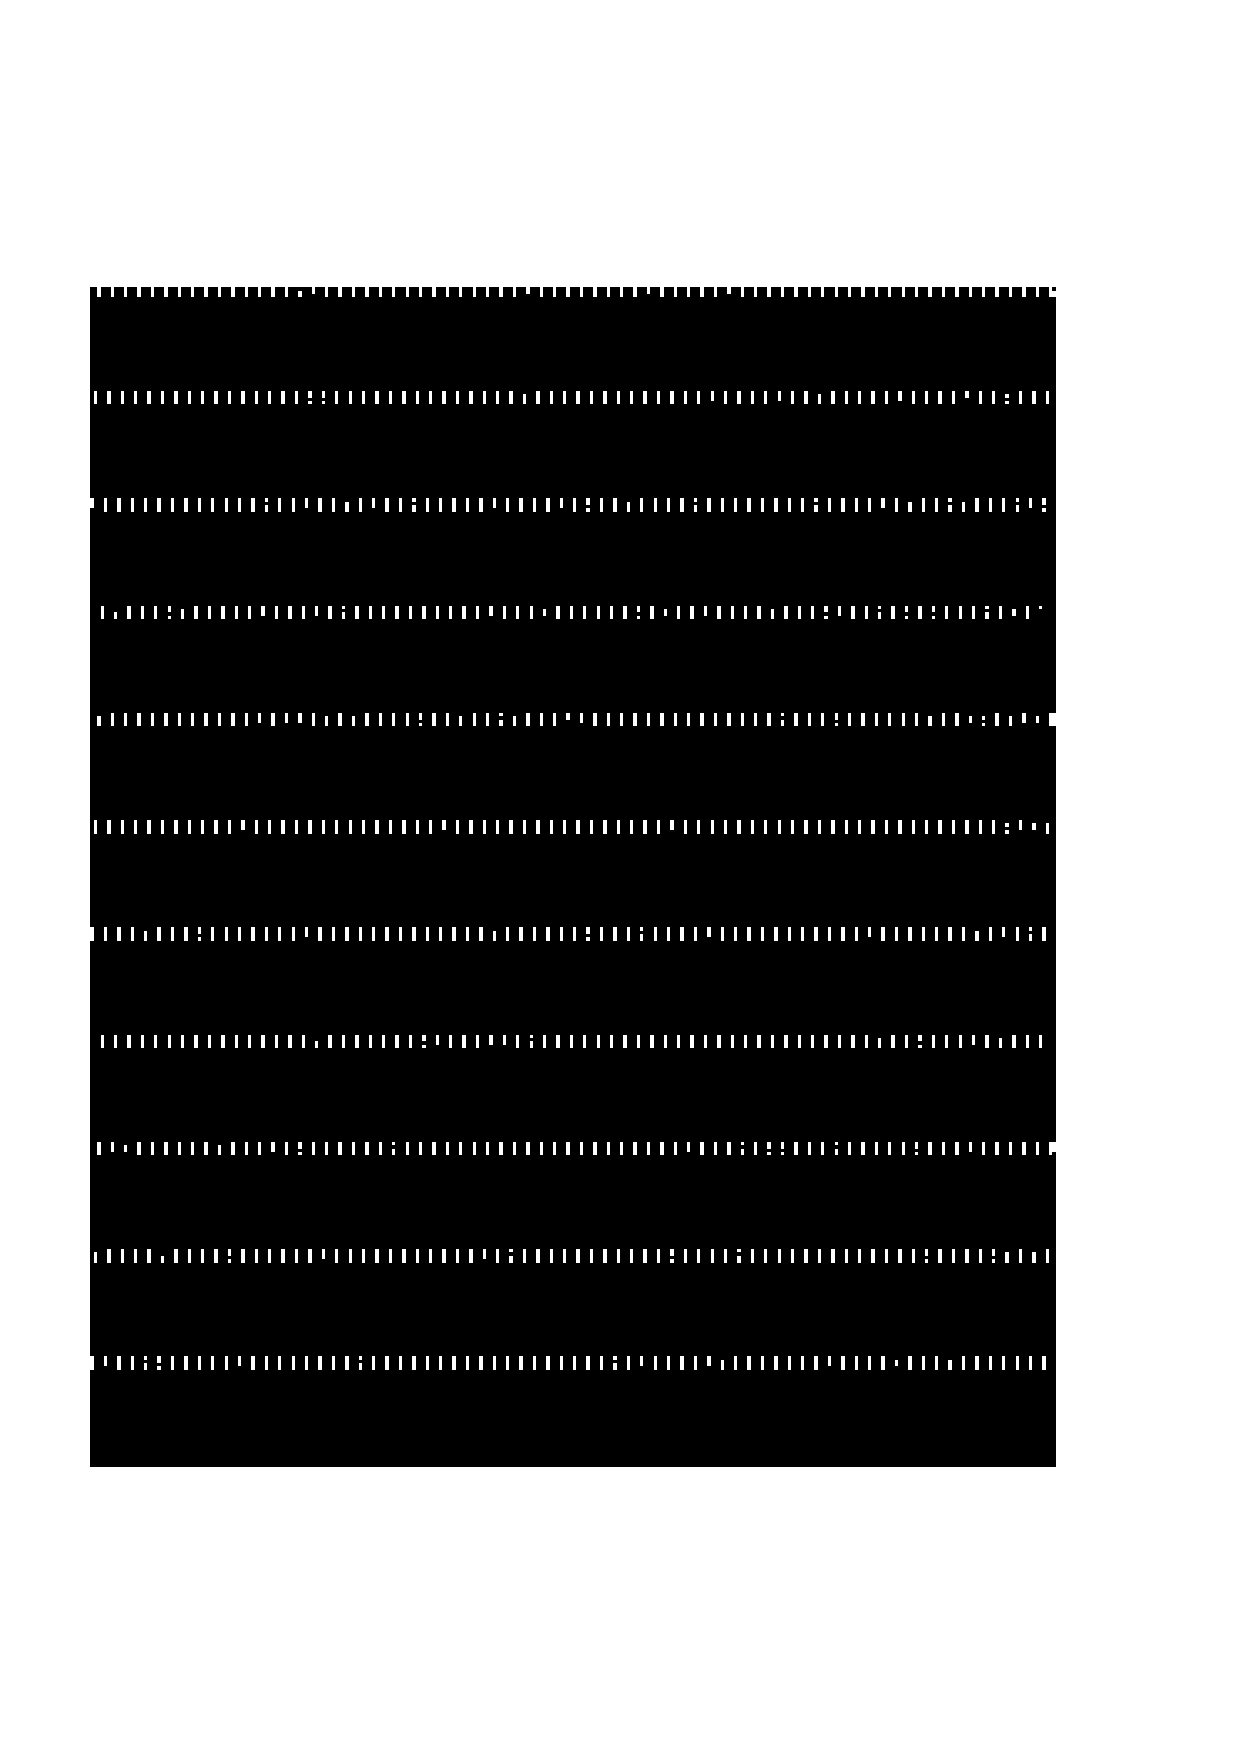
\includegraphics[width=0.5 \textwidth, angle=90]{burst_err.pdf}
	\caption{Image of burst optimization errors}
	\label{fig:pic_burst_err}
\end{figure}